\documentclass[12pt, titlepage]{article}
\usepackage{xcolor} % for different colour comments

%% Comments
\newif\ifcomments\commentstrue

\ifcomments
\newcommand{\authornote}[3]{\textcolor{#1}{[#3 ---#2]}}
\newcommand{\todo}[1]{\textcolor{red}{[TODO: #1]}}
\else
\newcommand{\authornote}[3]{}
\newcommand{\todo}[1]{}
\fi

\newcommand{\wss}[1]{\authornote{magenta}{SS}{#1}}
\newcommand{\ds}[1]{\authornote{blue}{DS}{#1}}

%% Graphics
\usepackage{float}
\usepackage{caption}
\usepackage{graphicx}
\graphicspath{ {Images/} }

\begin{document}

\title{Smart Waiter Detailed Design} 
\author{Meraj Patel \#1137491 \\ Pavneet Jauhal \#1149311\\ Shan Perera \#1150394}
\date{\today}
\maketitle

\tableofcontents 

\listoffigures

\listoftables


\pagebreak

\section{Introduction}

\ds{Why include this if it's identical to your SA introduction?}

\subsection{Purpose}
The purpose of Smart-Waiter aims to provide a solution that will allow users to order and pay through a mobile application at restaurants.

\subsection{Description}
This opportunity arose from the lack of a universal application in the market that allows users to walk into a restaurant, scan a code to view the menu, and proceed to order and pay through the use of a singular application. Android users will be able to walk into any restaurant that offers our solution, and have the ability to use these services.

\subsection{Scope}
The scope of Smart-Waiter will be limited to providing the user with the following features: viewing the restaurant's menu, creating the user's order, placing the order and paying for their order. 

\section{Overview}
\subsection{Revision History}

\begin{table}[H]
\begin{tabular}{|c|c|}
\hline
\textbf{Date}  & \textbf{Comments} \\ \hline
January 11, 2016 &  First Draft. \\ 
\hline
\end{tabular}
\caption{Revision History Table}
\end{table}

\section{Development Details}
\subsection{Language of Implementation}
The source code of the Android Smart-Waiter application will be written in Java and XML, as well as the API libraries used in development. 

\subsection{Supporting Frameworks/APIs}
CouchbaseLite (Database)\\
ZXing Embedded (QR Code Scanner)\\
Stripe (Credit Card)

\section{Implementation Components}
\subsection{Camera Function}
In this section we will detail the function that relates to the camera aspect of Smart-Waiter. There is one main function necessary for QR code scanning: onActivityResult. onActivityResult is called as soon as a QR code is captured by the camera. The function is passed three variables, a requestCode (int), a resultCode (int), an intent (Intent). Using these three variables, the function calls the ZXing function parseActivityResult using the three aforementioned variables as parameters. The parseActivityResult returns the contents of the QR code. 
 
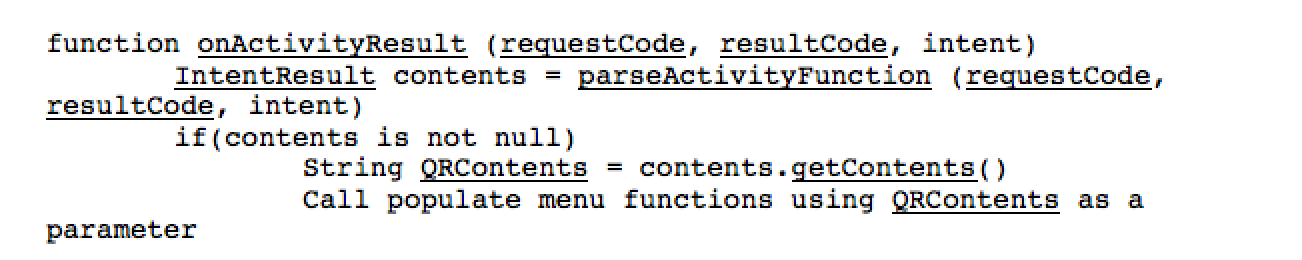
\includegraphics[width=150mm,scale=0.5]{camera.png}

\subsection{Account Function}
In this section we will detail the key function that relates to account transactions and credit card charges. There is one key method related to credit card transactions: chargeParams, it involves using the Stripe class. As described in the System Architecture, given an instance of the Card class, and using Smart-Waiter's Stripe API key, a token is created and sent to the Stripe servers. The Stripe servers return a token that can be used to charge the user's credit card. The token is then used as a parameter of chargeParams, along with the information related to the credit card charge, like amount and the type of currency. 

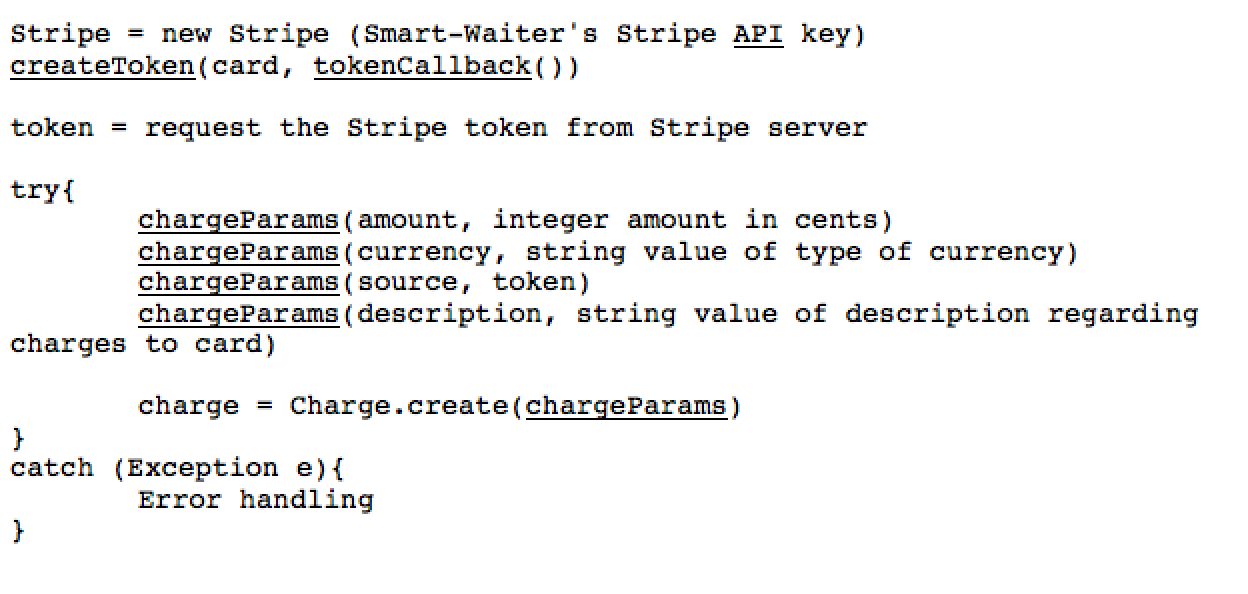
\includegraphics[width=150mm,scale=0.5]{stripe.png}

\subsection{Ordering Functions}
Below are function descriptions that are necessary for ordering in Smart-Waiter. As explained in System Architecture, there are three primary classes used to hold all vital information regarding menu information. These are: MenuCategories, MenuItems and User. These three classes are used to provide a user with a full menu of a particular restaurant and allow them to place an order.

\subsubsection{Parsing Function}
A parsing function was created to parse through received JSON responses to save information in appropriate classes. Stated below is pseudo code for this JSON parser. This function will parse through a JSON request. View if the key equals "categoryname". If so, save the value within MenuCategories class under variable, categoryName. Also, if the key equals "categorypic" save the value within MenuCategories class under variable, categoryPic.

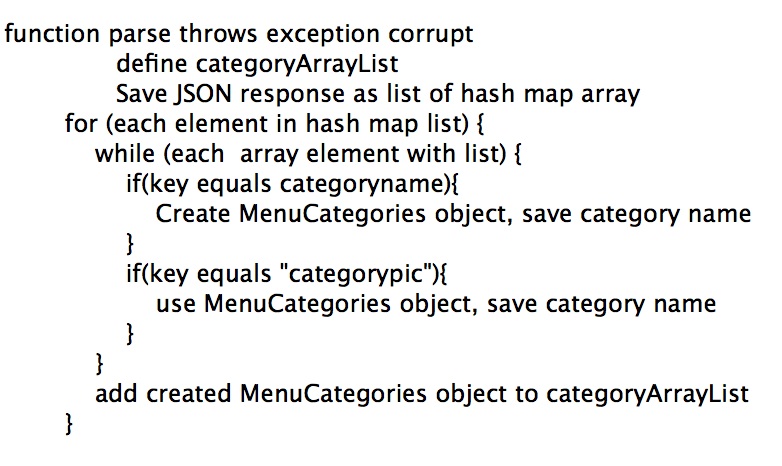
\includegraphics[width=150mm,scale=0.5]{parser.png}


\subsubsection{MenuCategories functions}
Primary functions are accessors and mutators
\begin{description}
  \item[getCategory:] Get category name
  \item[getPic:] Get category picture
\end{description}

\subsubsection{MenuItems functions}
Primary functions are accessors and mutators
\begin{description}
  \item[getItemName:] Get item name
  \item[getItemDetail:] Get item description
  \item[getItemPrice:] Get item price 
\end{description}

\subsubsection{Users functions}
Primary functions are accessors and mutators
\begin{description}
  \item[requestCode:] Used to parse the QR code 
  \item[resultCode:] Used to parse the QR code 
  \item[intent:] Gives the current intent, used to parse the QR code
\end{description}

\subsection{Couchbase Functions}

\subsubsection{Creating local database}
A top-level manager object is created when the application launches, which manages collection of couchbase instances. In the case of this application, there are two database instances, one that holds menus and another to hold orders. The Manager creates a directory in the filesystem (if one does not already exist) and stores the databases inside it. The file path is determined by the application context. Thus, if the application is ever deleted, all of the content will be deleted as well. In addition, creating the database at this point makes it readily available for functions, which might try to use it immediately following the application’s launch. 

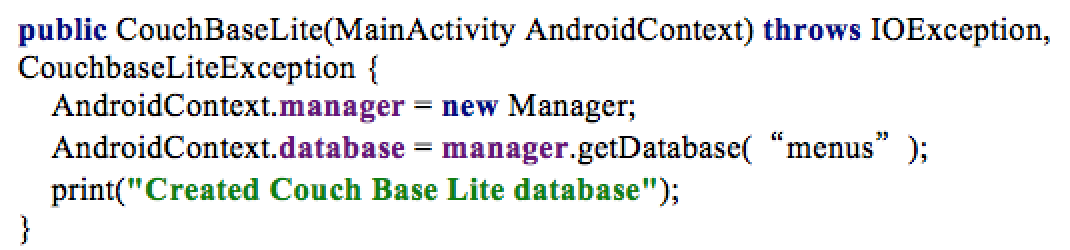
\includegraphics[width=150mm,scale=0.5]{createDatabase.png}

\subsubsection{Creating local database}
The CouchbaseLite API is used to access the documents by barcode. Furthermore, the couchbase get API is used to extract all menu details. An example of extracting a menu from the database is given below.

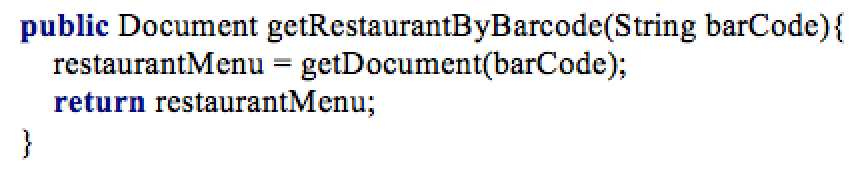
\includegraphics[width=150mm,scale=0.5]{accessdatabase.png}

\subsubsection{Replications}
Couchbase API will be used to replicate data from the cloud. For the scope of the application a replication of the whole database is used. However, in the future when there are thousands of restaurants, a filter can be used to pull specific menus from the cloud on demand. Both a continuous pull and push sync are setup so the application can push and pull at any time the application is running. In addition, a change listener is set on each pull to confirm the status. 

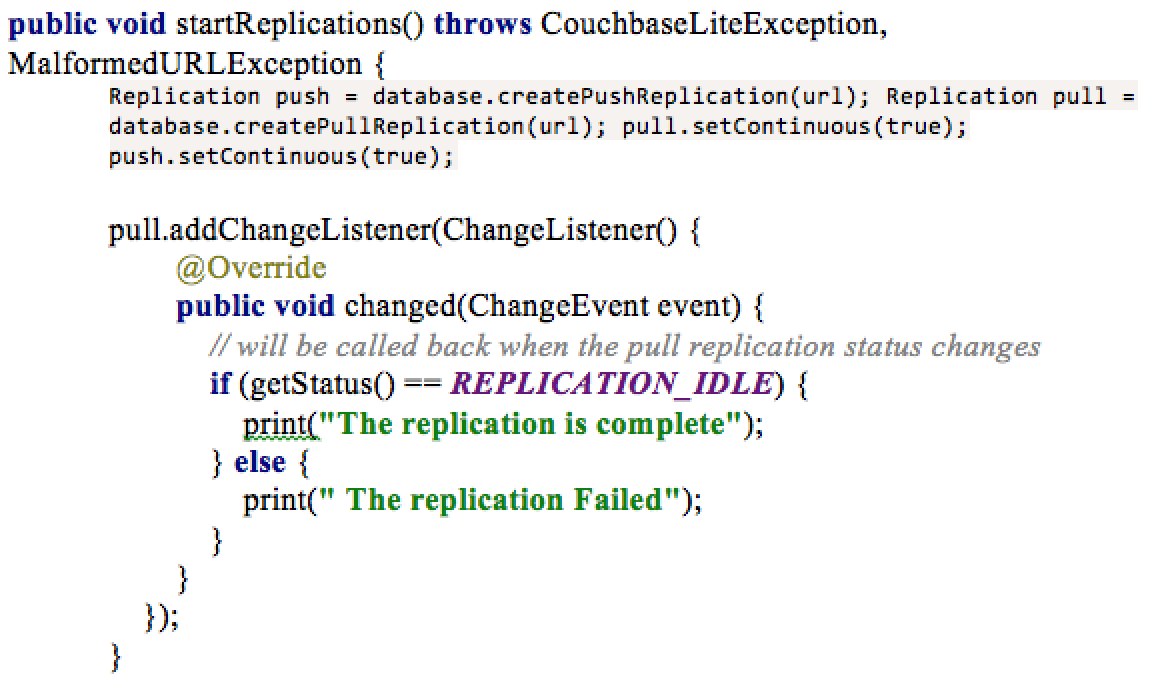
\includegraphics[width=150mm,scale=0.5]{replications.png}

\subsubsection{Sync Gateway}

The Sync Gateway requires some basic configuration to correctly synchronize mobile devices and the Couchbase server. The basic configuration is given below. Firstly, the sync gateway is pointed towards the Couchbase server node and the data bucket, which holds menus and orders. Furthermore, the Sync gateway is assigned a “sync data” bucket. This bucket is necessary because the sync gateway needs to store meta-data for accessed documents, such as revision etc. Since we want to decouple the sync-gateway from the Couchbase server and the restaurant menu’s and orders data. A new bucket is created for storing sync gateway metadata. 

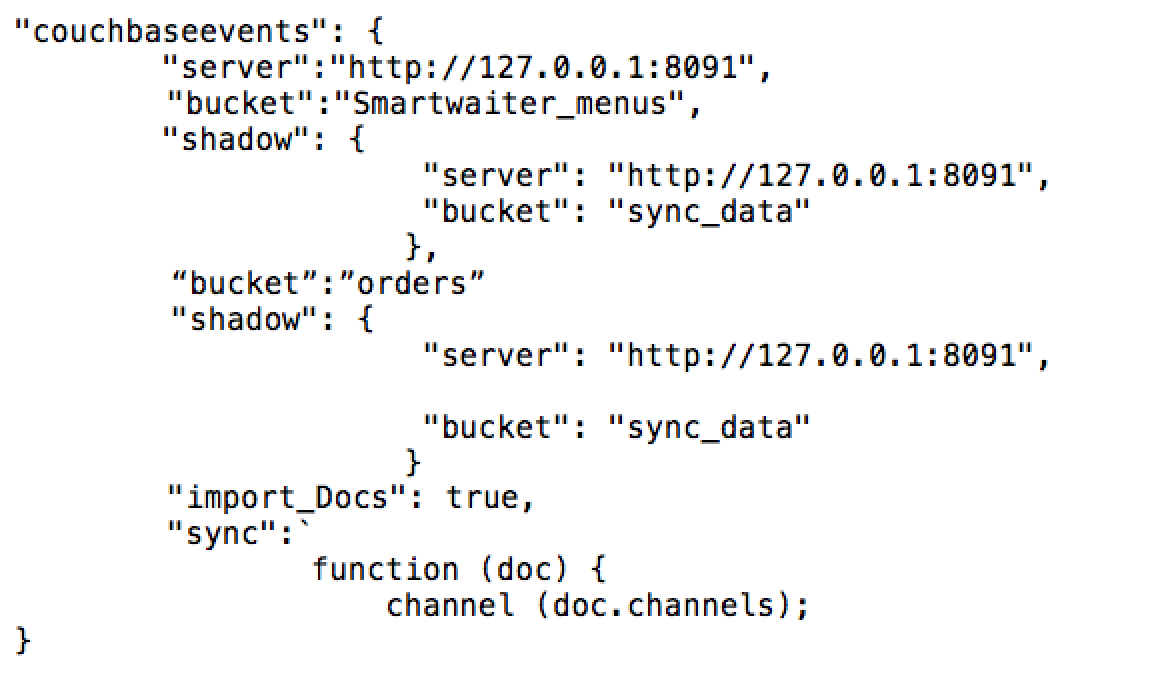
\includegraphics[width=150mm,scale=0.5]{jsonCouchbase.png}

\subsection{Error Handling}

As per the pseudo code, functions throw appropriate exception when an error occurs. There will actually be an error-handling module called in the catch statement, which will handle all of the error in the program.  The design will be a simple mapping between error code and how the error will be handled. In some cases for instance, when scanning an invalid barcode, the error is handled by propagating the error to the UI. Similarly, error which result in unexpected behavior will be propagated up to the UI. However, other errors such as replication fail due to network connectivity could be ignored and logged in the application log dump for debugging. They will not be propagated up to the UI. This module will most likely be changed according to feedback from end users.

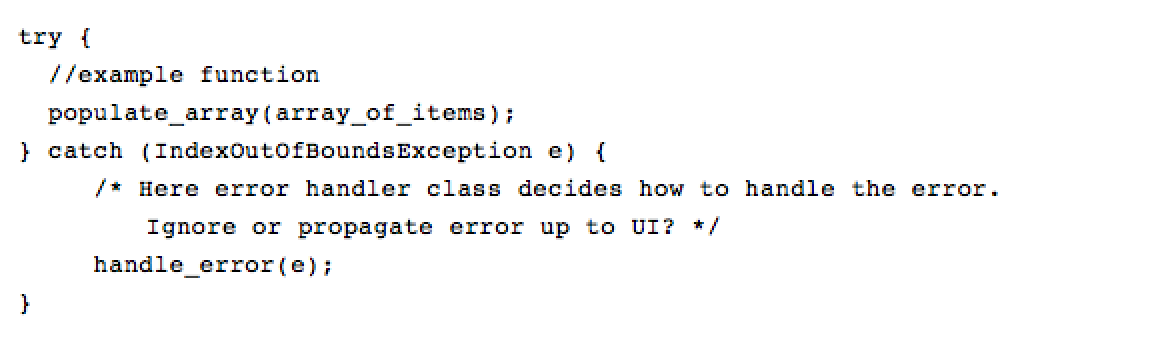
\includegraphics[width=150mm,scale=0.5]{error.png}

\subsection{Communication Protocol}
There is only one communication protocol used within server-client inside of our application. This is used to pull information from the couchbase server. However, the application simply calls Couchbase Lite API to pull data from the server. The details are implemented by couchbase Lite class itself.  An example of HTTP get is given below to pull data from server using a Mac terminal. 

curl -X GET 192.168.2.12:4984/couchbaseevents/1

\section{Database Structure}

\subsection{Implementation detail}
The couchbase server uses some basic rules to store data on the cloud. Here are some of the following:
\begin{itemize}
  \item Data is stored as key-value pairs, where the key is the barcode and the value is the entire menu of the restaurant.
  \item Buckets are basically equivalent of a database.
  \item Each item in the database is referred to as a document.
  \item The database is schema-less, thusly
	\ds{``thus"}
   there is no rigid structure
\end{itemize}

\subsection{JSON data format}
As mentioned above the database is schema less, meaning the JSON format and attributes can change from one restaurant to another. However below is an overview of the general JSON formatted restaurant menu.

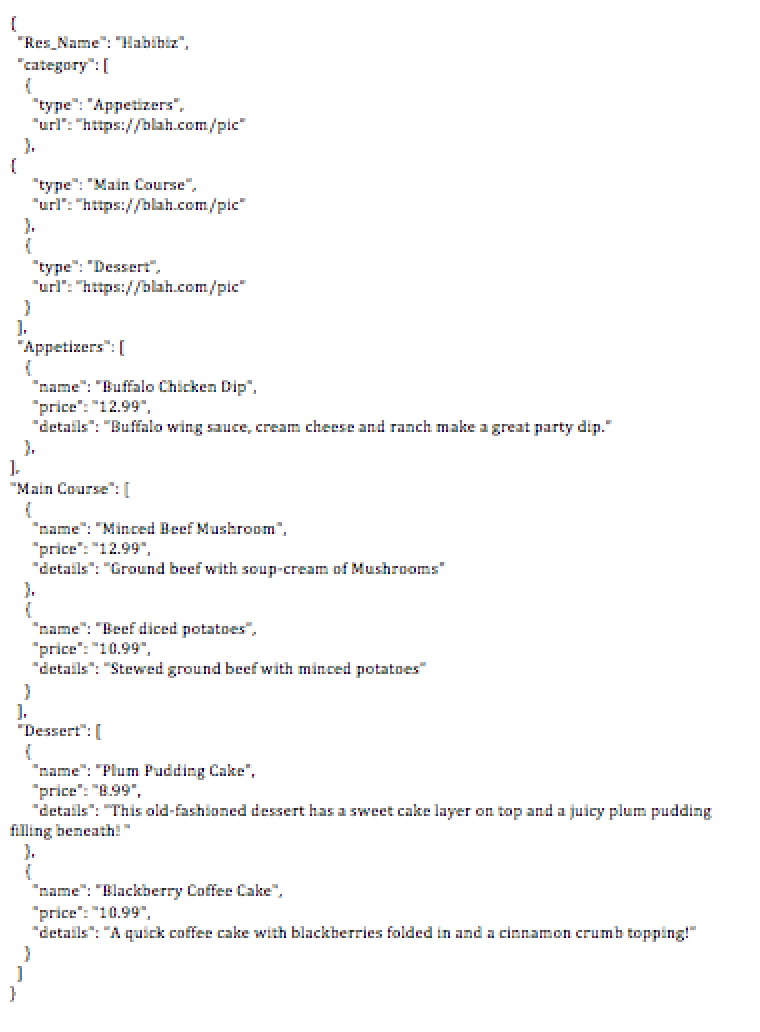
\includegraphics[width=150mm,scale=0.5]{JSONdata.png}


\section{User Interface Design}

\subsection{User Interface Design Overview}
Below are sample screen mock ups for the UI in place for Smart Waiter

\subsubsection{Menu Categories}
\begin{figure}[H]
\centering 
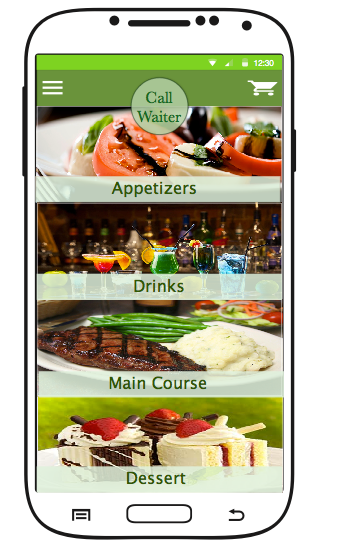
\includegraphics[width=80mm,scale=0.5]{MenuCategories.png}
\caption{Main menu UI screen}
\end{figure}
\subsubsection{Menu Items}

\begin{figure}[H]
\centering 
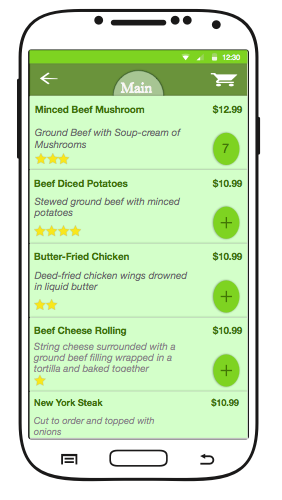
\includegraphics[width=80mm,scale=0.5]{CategoryItems.png}
\caption{Entree Category UI screen}
\end{figure}

\subsubsection{Confirm Order}
\begin{figure}[H]
\centering
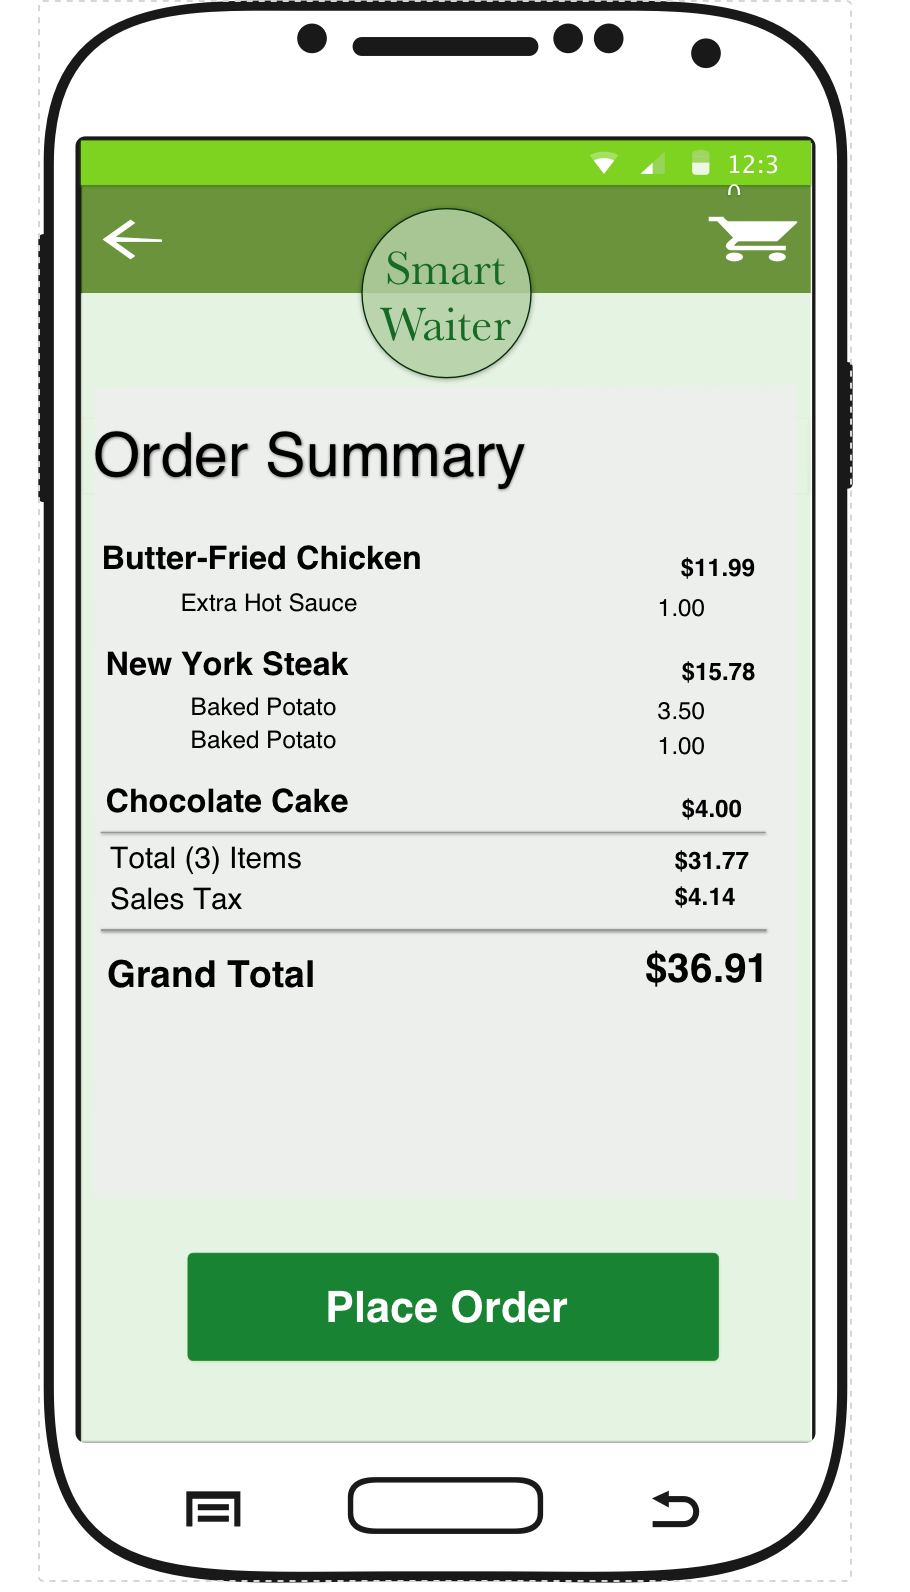
\includegraphics[width=80mm,scale=0.5]{OrderSummary.png}
\caption{Order Confirmation UI screen}
\end{figure}

\subsection{User Interface Navigation Flow}
Presented is the over all UI navigation flow for Smart Waiter. Provided below are descriptions and use cases of each component. 

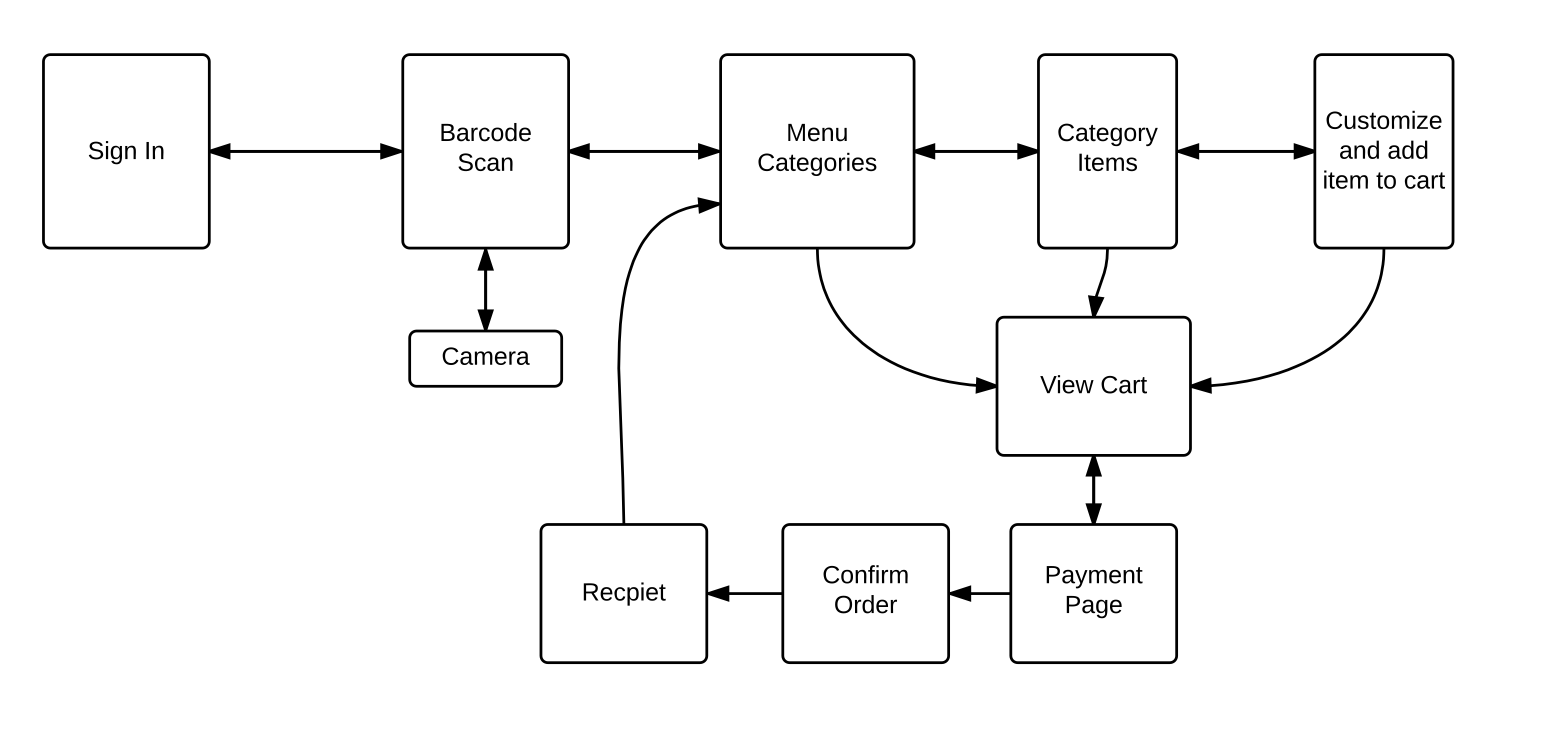
\includegraphics[width=180mm,scale=0.5]{UIProcess.png}

\subsection{UI Description and Use Cases}

\subsubsection{Sign In Page}

When the app 
\ds{``application"}
is launched the user is presented a screen promoting to sign in or skip sign in. The app will transition to one of two screens depending on the user’s decision. If the user decides to sign in, he will be redirected to a sign in page. Else, if he chooses to skip sign in, he will be redirected to barcode scanning page.


\begin{center}
    \begin{tabular}{ | l | p{8cm} |}
    \hline
    User Input & System Response \\ \hline
    Enters correct user name and password & Application transitions to Barcode Scan page \\ \hline
    Enters incorrect user name and password & Toaster displayed reading "incorrect login, please try again" \\ \hline
    Enters incorrect user name & Toaster displayed reading "incorrect login, please try again" \\ \hline
    Enters incorrect password & Toaster displayed reading "incorrect login, please try again" \\ \hline
    Clicks "Skip Sign in" & Application  transitions to Barcode Scan page\\ \hline
    Clicks Back Button on phone & Application Quits \\
    \hline
    \end{tabular}
\end{center}


\subsubsection{Barcode Scan Page}

This page informs the user to locate the barcode presented on the table in front of him in the restaurant.  After doing so, the user is asked to click “Scan”, to scan the bar code. Doing so, the app will transition to the camera page so the user can scan the code. Successfully scanning the barcode will transition to menu categories page. 

\begin{center}
    \begin{tabular}{ | l | p{10cm} |}
    \hline
    User Input & System Response \\ \hline
    Clicks Scan Barcode & Application transitions to camera so user can scan code. If successful, application will transition to menu page. Otherwise will return to scanning page and display a toaster reading, "please try again" \\ \hline
    Clicks back button on phone & Application transitions to Sign in Page \\
    \hline
    \end{tabular}
\end{center}

\subsubsection{Menu Categories Page}
This page display menu categories in wide labels that cover the screen. Attached is the category name and a picture above. An example can be seen in 6.1.1. A user would simply click on a category to view its menu items. Doing so will transition the app to Category Items Page. 

\begin{center}
    \begin{tabular}{ | l | p{10cm} |}
    \hline
    User Input & System Response \\ \hline
    Clicks category & Application transitions Category Items \\ \hline
    Clicks back button on phone & Application transitions to Barcode Scan \\
    \hline
    \end{tabular}
\end{center}

\subsubsection{Category Items Page}
This page display menu items in an android list view. Within each cell contains the item name, description and price. A use would simply tap on a cell to customize the item and add to cart. Please see 6.1.2 for an example.

\begin{center}
    \begin{tabular}{ | l | p{10cm} |}
    \hline
    User Input & System Response \\ \hline
    Clicks Item & Application transitions to Customize Item \\ \hline
    Clicks back button on phone & Application transitions to Menu Categories \\
    \hline
    \end{tabular}
\end{center}


\subsubsection{Customize Item Page}
This page allows customization of menu item. The UI consists of check boxes and options to indicate if certain toppings want to be added. The format of page is dependent on the type of item. At the bottom of the page, there will always be an option to add item to cart. 

\begin{center}
    \begin{tabular}{ | l | p{8cm} |}
    \hline
    User Input & System Response \\ \hline
    Ticks check boxes & None \\ \hline
    Enters special instructions in input field & None \\ \hline
    Clicks "Add to Cart" & Transitions to cart page and populate list with item \\ \hline
    Clicks back button on phone & Application transitions to Menu items \\
    \hline
    \end{tabular}
\end{center}

\subsubsection{Cart Page}
This page displays all menu items a user requested. Below is an option to submit the order and proceed to payment page. 
\begin{center}
    \begin{tabular}{ | l | p{10cm} |}
    \hline
    User Input & System Response \\ \hline
 	Clicks "Delete" &  Deletes item from list\\ \hline
    Clicks "Submit Order" &  Transitions to payment page\\ \hline
    Clicks back button on phone & Application transitions to previous page \\
    \hline
    \end{tabular}
\end{center}

\subsubsection{Payment Page}
This page allows users to input credit card information. This is the final page of the UI. After processing transaction, user will be redirected to bar code scan page. 
\begin{center}
    \begin{tabular}{ | l | p{7cm} |}
    \hline
    User Input & System Response \\ \hline
 	Input valid credit card and clicks "Process" & Transitions into Confirm Order page \\ \hline
    Input invalid credit card and clicks "Process" &  Toaster displayed reading "invalid credit card"\\ \hline
    Clicks back button on phone & Application transitions to previous Cart Page \\
    \hline
    \end{tabular}
\end{center}



\end{document}
